\documentclass[aspectratio=169]{beamer}

% -------------------- Theme --------------------
\usetheme{CambridgeUS}
\usecolortheme{dolphin}

% -------------------- Packages --------------------
\usepackage[utf8]{inputenc}
\usepackage[T1]{fontenc}
\usepackage[french]{babel}
\usepackage{graphicx}
\usepackage{amsmath}
\usepackage{emoji}

% -------------------- Fonts & spacing --------------------
\setbeamertemplate{itemize item}{\small$\blacktriangleright$}
\setbeamertemplate{itemize subitem}{\tiny$\bullet$}
\setbeamertemplate{footline}[default]
\setbeamertemplate{footline}{}

% -------------------- Title --------------------
\title{Analyse critique des stratégies de distribution des CNN en IoT}
\author{Supervisé par : AIT OMAR Driss\\
            Préparé par : AIT AHMED OULHAJE Soulaimane}
\institute{Master AIDC — FST Béni Mellal}

% -------------------- Document --------------------
\begin{document}

% -------------------- Title --------------------
\begin{frame}
  \titlepage
\end{frame}

% =================================================
% =================================================
% =================================================
\begin{frame}{Contexte : Inférence CNN en environnements IoT}

\begin{itemize}

    \item \textbf{CNN sont aujourd’hui largement utilisés}
    \begin{itemize}
        \item pour vision intelligente, surveillance, santé connectée
        \item traitement de données issues de caméras, capteurs et dispositifs mobiles
    \end{itemize}

    \bigskip

    \item \textbf{Dispositifs sont fortement contraints en}
    \begin{itemize}
        \item architectures matérielles différentes
        \item capacités de calcul variables
        \item contraintes mémoire et énergétiques importantes
    \end{itemize}

    \bigskip

    \item \textbf{Ce qui rend difficile}
    \begin{itemize}
        \item l’exécution complète d’un CNN est souvent impossible sur un seul device IoT
        \item les CNN modernes contiennent un grand nombre de paramètres
        \item nécessitent des ressources GPU/CPU importantes
    \end{itemize}

\end{itemize}
\end{frame}

% =================================================
\begin{frame}{Les solutions Cloud et Edge présentent chacune des limites}

\begin{itemize}

    \item \textbf{Limites du traitement Cloud}
    \begin{itemize}
        \item transmission complète des données vers des serveurs distants
        \item augmentation de la latence réseau
        \item surcharge du trafic de communication
        \item risques liés à la confidentialité des données
    \end{itemize}

    \bigskip

    \item \textbf{Limites du traitement Edge}
    \begin{itemize}
        \item réduction de la latence réseau
        \item traitement local proche des données
        \item limitation par les ressources matérielles locales
        \item difficulté à exécuter des CNN complexes
    \end{itemize}

\end{itemize}

\begin{block}{Conclusion}
    Cela motive l’étude de stratégies de distribution permettant de mieux exploiter les ressources disponibles tout en garantissant performance et sécurité.
\end{block}

\end{frame}

% =================================================
\begin{frame}{Distribution par Feature Maps (Approche de l’article)}

\begin{columns}[T] % Alignement en haut

    % Colonne gauche : image
    \begin{column}{0.55\linewidth}
        \centering
        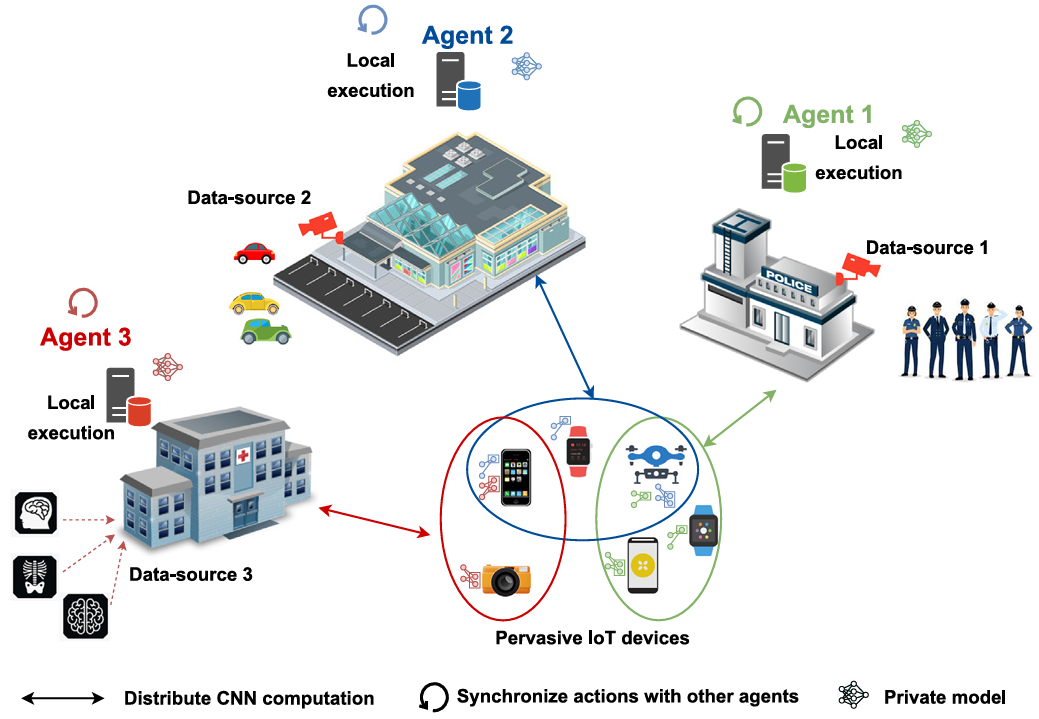
\includegraphics[width=\linewidth,height=0.55\textheight,keepaspectratio]{figures/distSys.png}
    \end{column}

    % Colonne droite : texte
    \begin{column}{0.45\linewidth}
        \begin{itemize}
            \item Chaque couche CNN génère plusieurs feature maps
            \item Ces feature maps peuvent être partitionnées
            \item Chaque dispositif IoT traite un sous-ensemble des sorties
        \end{itemize}
    \end{column}

\end{columns}

\smallskip

\begin{block}{Principe}
Les feature maps produites par une même couche CNN sont considérées comme des unités de calcul indépendantes, pouvant être distribuées entre plusieurs dispositifs IoT afin de paralléliser l’inférence.
\end{block}

\end{frame}



% =================================================
\begin{frame}{Pourquoi cette hypothèse est irréaliste}

\begin{block}{Corrélation entre feature maps et apprentissage conjoint}
Dans un CNN, les feature maps d’une même couche sont apprises de manière
conjointe et présentent une forte interdépendance.
\end{block}

\bigskip

\begin{itemize}
    \item Dans une couche convolutionnelle :
    \begin{itemize}
        \item chaque filtre parcourt \textbf{toutes les feature maps d’entrée}
        \item le filtre combine ces informations pour produire \textbf{une seule feature map de sortie}
    \end{itemize}
        \item Chaque filtre est optimisé pour détecter un type spécifique de motif
\end{itemize}

\begin{alertblock}{Conclusion critique}
\begin{itemize}
    \item Cela signifie que les feature maps sont fortement dépendantes entre elles.
    \item Leur séparation casse la logique du modèle CNN.
\end{itemize}
\end{alertblock}

\end{frame}

% =================================================
\begin{frame}{Distribution par couche (RL-PDNN)}

\begin{columns}

    % Colonne gauche : illustration
    \begin{column}{0.45\linewidth}
        \centering
        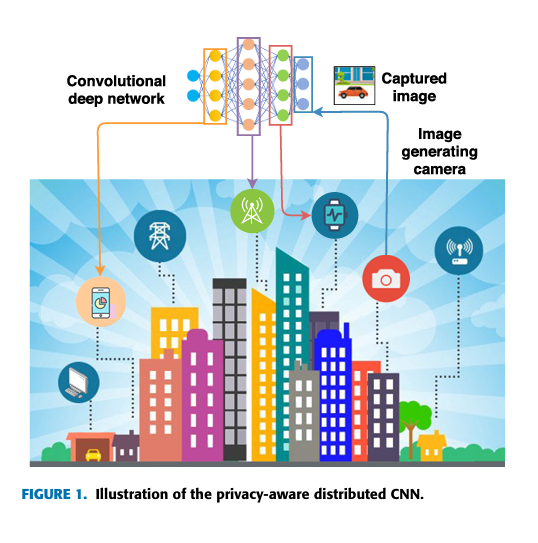
\includegraphics[width=\linewidth]{figures/Rep_CNN_1.png}
    \end{column}

    % Colonne droite : description
    \begin{column}{0.55\linewidth}
        \begin{itemize}
            \item Chaque couche CNN est exécutée intégralement sur un seul dispositif
            \item La stratégie de distribution est \textbf{dynamique} et pilotée par un agent de Reinforcement Learning
            \item Limitation de l’exposition structurelle du modèle CNN
            \item Contrairement à la distribution par feature maps, cette approche conserve l’intégrité fonctionnelle des couches CNN, tout en adaptant dynamiquement leur placement aux contraintes des dispositifs IoT.
        \end{itemize}
    \end{column}

\end{columns}

\end{frame}

% =================================================
\begin{frame}{Limites de la distribution par couche}

\begin{itemize}
    \item Le device observe une relation entrée--sortie cohérente
    \item Système reste vulnérable aux attaques \textit{black-box}, basées sur l’observation des entrées et des sorties.
    \item La distribution par couche limite l’accès aux paramètres internes, Ce qui renforce la protection contre les attaques \textit{white-box} (attaquant possède un accès complet au modèle)
\end{itemize}

\end{frame}




% ==================================================
\begin{frame}{Formulation du problème (Formule détaillée)}

\textbf{Objectif global}

\medskip
Cette formule représente la fonction objectif de notre problème d’optimisation :
\small
\[
\min_{A}
\sum_{r^* \in \mathcal{RQ}}
\sum_{i \in \mathcal{I} \cup \mathcal{S}}
\sum_{j \in \mathcal{I} \cup \mathcal{S}}
\sum_{l=1}^{L_{n_{r^*}}-1}
A^{i}_{r^*,l} \cdot A^{j}_{r^*,l+1}
\cdot
\frac{O^{l}_{r^*}}{\rho_i}
\cdot \mathbf{1}_{i \neq j}
\;+\;
\sum_{i \in \mathcal{I} \cup \mathcal{S}} t_i^{c}
\]
\medskip
Elle vise à :
\begin{itemize}
    \item minimiser la latence totale,
    \item La fonction somme ces coûts pour toutes les couches et pour toutes les requêtes CNN arrivant dans le système.

    \item  Ainsi, le problème consiste à déterminer sur quel dispositif exécuter chaque couche du CNN afin de minimiser la latence globale tout en respectant les contraintes du système IoT.
\end{itemize}


\end{frame}

% -------------------- Slide --------------------
\begin{frame}{Premier terme : coût de communication}

\small
\[
\sum_{r^* \in \mathcal{RQ}}
\sum_{i \in \mathcal{I} \cup \mathcal{S}}
\sum_{j \in \mathcal{I} \cup \mathcal{S}}
\sum_{l=1}^{L_{n_{r^*}}-1}
A^{i}_{r^*,l} \cdot A^{j}_{r^*,l+1}
\cdot
\frac{O^{l}_{r^*}}{\rho_i}
\cdot \mathbf{1}_{i \neq j}
\]

\medskip
\begin{itemize}
    \item Il apparaît lorsque deux couches consécutives du CNN sont exécutées sur deux dispositifs différents.
    \item introduit une latence de transmises dépendant du volume des données et du débit du réseau.
    \item $\frac{O^l_r}{\rho_i}$ : temps de transmission des données intermédiaires
\end{itemize}

\medskip
Ce terme :
\begin{itemize}
  \item mesure le coût de communication induit par la distribution du CNN,
  \item pénalise les allocations qui fragmentent excessivement les couches.
\end{itemize}

\end{frame}

% -------------------- Slide --------------------
\begin{frame}{Deuxième terme : coût de calcul}

\[
\sum_{i \in \mathcal{I}} t_i^c
\qquad \text{avec} \qquad
t_i^c =
\sum_{r}
\sum_{l}
A^{i}_{r^*,l} \cdot \frac{c^l_r}{e(i)}
\]

\medskip
\begin{itemize}
  \item Ce coût dépend de la puissance de calcul du device et du nombre de couches qu’il exécute.
  \item $c^l_r$ : charge de calcul de la couche
  \item $e(i)$ : puissance de calcul du device $i$
\end{itemize}

\medskip
Ce terme :
\begin{itemize}
  \item pénalise l’utilisation de dispositifs à faible puissance,
  \item favorise une répartition équilibrée de la charge de calcul.
\end{itemize}

\end{frame}

\begin{frame}{Contraintes de ressources matérielles}
\textbf{Objectif :} garantir que chaque dispositif IoT dispose des ressources nécessaires pour exécuter les couches du CNN qui lui sont attribuées.

\vspace{0.3cm}
\begin{itemize}
    \item \textbf{Contrainte mémoire (a)} :
    \[
    \sum_{r \in RQ}\sum_{l}
    A^{i}_{r^*,l} \cdot m^{l}_{r^*}
    \le \bar{m}_i
    \]
    \small
    Elle assure que la somme de la mémoire requise par toutes les couches exécutées sur un dispositif ne dépasse pas sa capacité mémoire maximale.
    
    \vspace{0.2cm}
    \item \textbf{Contrainte de calcul (b)} :
    \[
    \sum_{r \in RQ}\sum_{l}
    A^{i}_{r^*,l} \cdot c^{l}_{r^*}
    \le \bar{c}_i
    \]
    \small
    Elle garantit que la charge computationnelle totale attribuée à un dispositif reste inférieure à sa capacité de traitement.
\end{itemize}
\end{frame}

\begin{frame}{Contraintes liées à la communication et à la cohérence}
\textbf{Objectif :} contrôler la latence réseau et assurer une
distribution cohérente des couches.

\vspace{0.3cm}
\begin{itemize}
    \item \textbf{Bande passante (c)} :
    \[
    \sum_{r,l,j}
    A^{i}_{r^*,l} A^{j}_{r^*,l+1}
    O^{l}_{r^*}
    \le \bar{b}^{d}_i
    \]
    \small
    Elle garantit que le volume total de données échangées entre les dispositifs IoT ne dépasse pas la capacité de communication disponible.

    \vspace{0.2cm}
    \item \textbf{Unicité de placement (d)} :
    \[
    \sum_{I_i} A^{i}_{r^*,l} = 1
    \]
    \small
    Chaque couche du CNN est exécutée sur un seul device.

\end{itemize}
\end{frame}

\begin{frame}{Contraintes liee au confidentialité et de décision}
\textbf{Objectif :} limiter les fuites d’information et garantir
des décisions claires.

\vspace{0.3cm}
\begin{itemize}
    \item \textbf{Indicateur d’exposition (g)} :
    \[
    H^{i}_{r^*,l} =
    \prod_{k=2}^{l-1}
    \max_{j} \left( A^{i}_{r^*,k} \right)
    \]
    
    \small
    Cet indicateur permet de vérifier si un dispositif a déjà exécuté des couches précédentes du CNN, qui peuvent contenir des informations sensibles sur la structure du modèle.

    \vspace{0.2cm}
    \item \textbf{Contrainte de confidentialité (h)} :
    \[
    1 - H^{i}_{r^*,l-1} \ge A^{i}_{r^*,l}
    \]
    \small
    Elle utilise l’indicateur d’exposition pour empêcher l’exécution de couches profondes sur des devices non
    autorisés (protection contre les attaques \textit{white-box}).
\end{itemize}

\vspace{0.2cm}
\centering
\textit{Ces contraintes encadrent la fonction objectif afin de
minimiser la latence tout en respectant les limites du système.}
\end{frame}

% =================================================
\begin{frame}{Transition vers l’implémentation}

\begin{block}{Motivation}
Après l’analyse critique des stratégies de distribution des CNN en IoT,
nous avons développé une première solution pratique basée sur
le \textbf{Reinforcement Learning mono-agent}.
\end{block}

\vspace{0.2cm}
\begin{itemize}
    \item Objectif : valider concrètement la distribution par couche
    \item Implémentation sous forme de preuve de concept
\end{itemize}

\vspace{0.2cm}
\begin{block}{Question centrale}
Comment décider intelligemment sur quel device exécuter
chaque couche du CNN afin de minimiser la latence globale ?
\end{block}

\end{frame}

% =================================================
\begin{frame}{Pourquoi le Reinforcement Learning ?}

\begin{itemize}
    \item Problème :
    \begin{itemize}
        \item combinatoire
        \item dynamique (ressources variables)
        \item difficile à résoudre par des règles fixes
    \end{itemize}
    
    \vspace{0.2cm}
    \item Le RL permet :
    \begin{itemize}
        \item un apprentissage par interaction
        \item l’optimisation d’une récompense globale
        \item une adaptation à différents scénarios IoT
    \end{itemize}
\end{itemize}

\end{frame}

% =================================================
\begin{frame}{Formulation RL : Agent et Environnement}

\textbf{Agent}
\begin{itemize}
    \item Un agent central mono-agent
    \item Décide du placement des couches du CNN
\end{itemize}

\vspace{0.2cm}
\textbf{Environnement}
\begin{itemize}
    \item Ensemble des devices IoT
    \item Capacités :
    \begin{itemize}
        \item puissance de calcul
        \item bande passante
        \item mémoire
    \end{itemize}
    \item Structure du CNN (LeNet5)
\end{itemize}

\end{frame}

% =================================================
\begin{frame}{États et Actions}

\textbf{État (State)}
\begin{itemize}
    \item index de la couche courante
    \item ressources disponibles des devices
    \item charge déjà assignée
    \item latence accumulée
\end{itemize}

\vspace{0.2cm}
\textbf{Action}
\begin{itemize}
    \item choix d’un device pour exécuter la couche suivante
\end{itemize}

\vspace{0.2cm}
\begin{block}{Interprétation}
Action = \textit{placer la couche $l$ sur le device $i$}
\end{block}

\end{frame}

% =================================================
\begin{frame}{Fonction de récompense et lien avec la formule math}

\textbf{Objectif du reward (Reinforcement Learning)}
\begin{itemize}
    \item Minimiser la latence globale du CNN distribué
    \item Pénaliser :
    \begin{itemize}
        \item la communication réseau entre devices
        \item les devices lents ou surchargés
        \item les violations de contraintes (mémoire, calcul)
    \end{itemize}
\end{itemize}

\[
r_i =
\begin{cases}
- R_{\text{penalty}}, & \text{si contraintes violées} \\
- \big( L_i^{\text{comp}} + L_i^{\text{trans}} \big), & \text{sinon}
\end{cases}
\]


\begin{block}{Lien avec la formule du PFE}
\begin{itemize}
    \item Le reward approxime la fonction objectif :
    \begin{itemize}
        \item coût de communication
        \item coût de calcul
    \end{itemize}
    \item Les contraintes sont intégrées sous forme de pénalités
\end{itemize}
\end{block}

\end{frame}

% =================================================
\begin{frame}{Vers une approche multi-agent}

\begin{itemize}
    \item Limite du mono-agent :
    \begin{itemize}
        \item décision centralisée
        \item faible passage à l’échelle (scalabilité : système devient plus grand)
    \end{itemize}

    \vspace{0.2cm}
    \item Extension naturelle :
    \begin{itemize}
        \item chaque source devient un agent autonome
        \item jeu coopératif / compétitif
    \end{itemize}
\end{itemize}

\begin{block}{Perspective}
MonoAgentRL constitue une base pour une future
implémentation multi-agent distribuée.
\end{block}

\end{frame}

% -------------------- Slide --------------------
\begin{frame}{Approches existantes en MARL}

\textbf{Approche 1 : Independent Q-Learning (IQL)}
\begin{itemize}
  \item Apprentissage \textbf{indépendant} de chaque agent
  \item Q-Learning / DQN appliqué localement
  \item Autres agents vus comme partie de l’environnement
  \item Pas de communication explicite
\end{itemize}

\textbf{Avantages :}
\begin{itemize}
  \item simple à implémenter
  \item scalable
  \item bien adapté aux systèmes IoT distribués
\end{itemize}

\bigskip

\textbf{Approche 2 : Centralized Training, Decentralized Execution (CTDE)}
\begin{itemize}
  \item Entraînement avec information globale
  \item Exécution décentralisée par agent
  \item Meilleure coordination entre agents
\end{itemize}

\textbf{Exemples :} QMIX, MADDPG, MAPPO

\end{frame}

\begin{frame}{Positionnement de notre approche}

\begin{itemize}
  \item L’IQL est utilisé comme approche de départ et \textbf{baseline expérimentale}.
  \item Dans notre implémentation, l’IQL est combiné avec des \textbf{réseaux de neurones profonds (DQN)}.
  \item Ce choix motivé par :
  \begin{itemize}
    \item simplicité de mise en œuvre
    \item faible complexité computationnelle
    \item adaptation aux environnements IoT distribués
  \end{itemize}
\end{itemize}

\bigskip
\textbf{Approche baseline pour le MARL profond}
\end{frame}

\begin{frame}{Independent Q-Learning avec DQN}

Chaque agent $i$ apprend indépendamment une fonction de valeur
approximée par un réseau de neurones :

\[
Q_i(s_i, a_i; \theta_i)
\]

\begin{itemize}
  \item $s_i$ : observation locale de l’agent, $a_i$ : action d’allocation du CNN, $\theta_i$ : paramètres du DQN
\end{itemize}

\bigskip

\textbf{Apprentissage}

\[
y_i = r_i + \gamma \max_{a_i'} Q_i(s_i',a_i';\theta_i^-)
\]

\[
L(\theta_i) =
\left(
y_i - Q_i(s_i,a_i;\theta_i)
\right)^2
\]

\begin{itemize}
  \item apprentissage indépendant par agent
  \item utilisation d’un réseau cible pour stabiliser l’apprentissage
\end{itemize}

\end{frame}

\begin{frame}{Implémentation IQL-DQN}

\textbf{Modélisation}

\begin{itemize}
  \item Chaque requête CNN est gérée par un agent DQN
  \item Observation :
  \begin{itemize}
    \item état partiel des ressources IoT et caractéristiques du CNN
  \end{itemize}
  \item Action :
  \begin{itemize}
    \item allocation des couches CNN sur les dispositifs IoT
  \end{itemize}
\end{itemize}

\bigskip

\textbf{Interaction avec l’environnement}

\begin{itemize}
  \item Les agents partagent un \textbf{Resource Manager}
  \item Chaque décision modifie les ressources système
  \item Environnement multi-agent non stationnaire
\end{itemize}

\bigskip

\textbf{Fonction de récompense}

\[
r_i =
\begin{cases}
- R_{\text{penalty}} & \text{si contraintes violées} \\
- (\text{latence calcul} + \text{latence communication}) & \text{sinon}
\end{cases}
\]

\end{frame}


\begin{frame}{Limites et perspectives de l’approche IQL}

\textbf{Limites}

\begin{itemize}
  \item absence de coordination explicite entre agents
  \item compétition implicite pouvant dégrader les performances
  \item convergence parfois lente dans des environnements non stationnaires
\end{itemize}

\bigskip

\textbf{Avantages}

\begin{itemize}
  \item simplicité de conception et d’implémentation
  \item robustesse en pratique
  \item bonne scalabilité dans les systèmes distribués
\end{itemize}

\bigskip

\textbf{Perspectives}

\begin{itemize}
  \item utilisation d’IQL comme baseline multi-agent
  \item étendu vers des approches coopératives :
  \begin{itemize}
    \item CTDE (QMIX, MAPPO)
    \item coordination et communication inter-agents
  \end{itemize}
\end{itemize}

\end{frame}

\end{document}